% Write the full path to the location of the graphics relative to book.tex
\graphicspath{{chapters/paratico/graphics/}}

\title{Estimation of optimal inlet boundary conditions for blood flow assessment in abdominal aortic aneurysm using variational data assimilation}
\titlerunning{Paratico et al.}

\author{S.~Paratico, R.~Munaf\`o, C.~Trenti, P.~ Dyverfeldt, S. Saitta and E.~Votta}
\authorrunning{Paratico et al.}

\institute{S.~Paratico \email{sara.paratico@mail.polimi.it} \at Politecnico di Milano}
\maketitle

\abstract{}
Blood fluid dynamics impacts vessel wall cells and tissue biomechanics, influencing thrombus formation and vessel wall remodeling. Accurate \textit{in vivo} quantification can thus aid in understanding these mechanisms and patient stratification. Computational fluid dynamics (CFD) and 4D flow magnetic resonance imaging (MRI) are used for this purpose, but both have limitations: CFD involves assumptions and boundary condition (BC) simplifications, while 4D flow MRI suffers from low spatial resolution and noise. This study employs variational data assimilation (VarDA) to integrate CFD and 4D flow MRI, yielding a high-resolution, noise-free flow field closely aligned with 4D flow MRI velocity data. To enhance alignment, the optimal inlet velocity profile is determined iteratively via an incremental pressure correction scheme (IPCS). Previously tested in simple synthetic geometries and later in a complex  patient-specific abdominal aortic aneurysm (AAA), this approach demonstrates improved reliability in patient-specific hemodynamic evaluation. 


\section*{Introduction}
Alterations in blood fluid dynamics often contribute to the progress of cardiovascular pathological conditions [\cite{Bappoo2021}, \cite{Guzzardi2015}]. Hence, quantifying blood fluid dynamics on a patient-specific basis and non-invasively can support the understanding of pathological mechanisms or the stratification of patients based on the risk for adverse endpoints. To this aim, blood flow field can be reconstructed from clinical imaging, namely 4D flow magnetic resonance imaging (MRI) [\cite{Dyverfeldt2015}], or computed through patient-specific computational fluid dynamics (CFD) models  [\cite{Kheyfets2015}]. 
However, 4D flow MRI provides indirect and noisy velocity measurements with low spatio-temporal resolution, which often violate mass conservation. CFD models solve discretized Navier-Stokes (NS) equations to compute well-resolved, noise-free velocity fields but are affected by numerical artifacts and rely on simplified boundary conditions (BCs), including inlet velocity BCs. Variational data assimilation (VarDA) integrates CFD-based NS equations with sparse, uncertain 4D flow MRI data by optimizing BCs to minimize discrepancies. In cardiovascular flows, it refines inlet velocity profiles but requires computing both velocity and pressure gradient fields, which is challenging in high-velocity arterial flows. Pressure-velocity coupling or correction schemes address this, yet MRI-induced noise can hinder proper pressure correction, affecting the accuracy of the solution.

\subsection*{Related works}
\label{sec:background}
Several studies have explored VarDA in hemodynamics, ranging from 2D steady-state to 3D transient conditions. \cite{Delia2012} showed that VarDA allows to reconstruct flow fields in geometrically complex 2D domains, such as the 2D representation of the aortic arch and carotid bifurcation, even with noisy velocity data. Subsequently, in \cite{Delia2013}, the same authors showed that, in 2D domains, noisy velocity data can be effectively managed by properly managing inlet BCs. In particular, they showed that the regularization of the inlet velocity profile through the use of a control variable also regularized the velocity field over the whole domain and allowed for successful pressure-velocity coupling. \cite{Tiago2017} extended VarDA to a 3D saccular aneurysm, demonstrating its flexibility with various BCs and optimization methods like gradient-based and genetic algorithms to improve accuracy. \cite{Koltukluoglu2018} showed that VarDA, applied to 4D Flow MRI data, outperformed traditional CFD methods by dynamically adjusting BCs in real-time to maintain flow congruence near inlets. \cite{Funke2019} demonstrated the effectiveness of 4D (3D space + time) VarDA in capturing transient blood flow in aneurysms using phase contrast-MRI data. Finally, \cite{Dokken2020} proposed a multimesh finite element (FE) method that enhanced stability and accuracy by allowing flexible BC management across multiple mesh domains, which is key for simulating complex hemodynamics in realistic geometries.

\subsection*{Aim of the work}
This study aims to implementing a method to compute \textit{in vivo} blood fluid dynamics on a patient-specific basis with high space-resolution without using simplifying hypotheses on the inlet BCs. To achieve this, VarDA is used to estimate an optimal inlet BC for CFD, starting from a noisy, uncertain 4D flow MRI-based velocity profile while enforcing consistency between the CFD-computed velocity field and sparse 4D flow MRI data in the bulk flow region. We benchmarked the method on ideal 2D and 3D geometries and then applied it to a patient-specific abdominal aortic aneurysm (AAA) geometry. 

\section*{Methods}
\label{sec:methods}

\subsection*{Data Assimilation Method}
The VarDA approach was formulated as an optimization problem constrained by the NS equations, using the \emph{dolfin-adjoint} library for the adjoint problem. The process follows three steps: running a first numerical simulation with tentative inlet BCs (which we refer to as the \emph{forward model} or \emph{Tape}), solving the optimization problem to identify inlet BCs, and running a final numerical simulation yielding the refined velocity and pressure fields (Fig. \ref{fig:scheme}).

\subsection*{Forward problem definition}
The weak and discretized form of NS equations for an incompressible fluid [\cite{Stokes2009}] was solved using the FE platform \emph{FEniCS} [\cite{Alnaes2015}] to compute velocity field $\textbf{u}$ over a domain $\Omega$ given an initial condition \(\mathbf{u}=\mathbf{u_0}\) on $\Omega$ at time $t_0$, a zero pressure condition at the outlet section $\Omega_N$ and a Dirichlet BC at the inlet section $\Omega_D$ in the form of a space- and time-dependent velocity profile $\textbf{g}$. Through an in house Python script, 2D and 3D fluid domains $\Omega$ were discretized into triangular and tetrahedral elements, respectively, with 1-1.5 mm characteristic size and with linear and quadratic shape functions for nodal pressure and velocity, respectively. The semi-implicit Crank-Nicolson (CN) time-integration scheme was applied with a time increment of $\Delta t = 0.001$ s. The incremental pressure correction scheme (IPCS) proposed in [\cite{Goda1979}] was implemented. A generalized minimal residual method (GMRES) was chosen as linear solver, with tolerances of $1 \times 10^{-4}$ for momentum and continuity equations.

\subsection*{Optimization Problem definition}

The optimization problem (\cref{eq:10}, constrained by the NS equations, aimed to minimize a functional $J(\mathbf{u})$ (\cref{eq:11}, defined as the difference between the computed and observed velocities. 

\begin{equation}
\small
\min_{\mathbf{c}} J(\mathbf{u}) + R(\mathbf{c}) \quad \text{s.t.} \quad F(\mathbf{u}, \mathbf{c}) = 0
\label{eq:10}
\end{equation}
\begin{equation}
\small
    J(\textbf{u}) = \| \mathbf{u} - \mathbf{u}_{\text{obs}} \|_{L^2(\Omega)}
    \label{eq:11}
\end{equation}

To address the ill-posedness of the problem, a Tikhonov regularization term $\textbf{R}(\textbf{c})$ was introduced, with respect to the controlled variable defined as $c$. It accounts for two terms that are scaled by parameters \(\alpha\) and \(\beta\), where \(\beta\) is set to $0$ for steady-state conditions. This reformulation transforms the problem into an unconstrained optimization scenario, more suitable for gradient descent methods. 

\begin{equation}
\small
    \begin{aligned}
        R(\mathbf{c}) &= \| \mathbf{c} \|_{L^2(\Omega)} \\
        &\text{where} \\
        \small
        \|c\|_{\Gamma \times (0, T]} &= \left( \int_0^T \int_{\Omega} \frac{\alpha}{2} \left( \left(|\textbf{g}_D|^2 + |\nabla \textbf{g}_D|^2 \right) + \frac{\beta}{2} \left( |\dot{\textbf{g}}_D|^2 +  |(\nabla \textbf{g})_D|^2 \right) \right) \, dx \, dt \right)^{\frac{1}{2}}
    \end{aligned}
    \label{eq:12} 
\end{equation}

The adjoint approach efficiently computes the total derivative of the functional, yielding the adjoint NS equations that facilitate optimization. The iterative Broyden-Fletcher-Goldfarb-Shanno (BFGS) algorithm, in its L-BFGS variant [\cite{Liu1989}], served as optimizer. The L-BFGS algorithm is already implemented in the SciPy library, which is automatically
called by dolfin-adjoint library and which provides many user-friendly numerical routines, such as the routine for optimization.


\begin{figure}
    \centering
    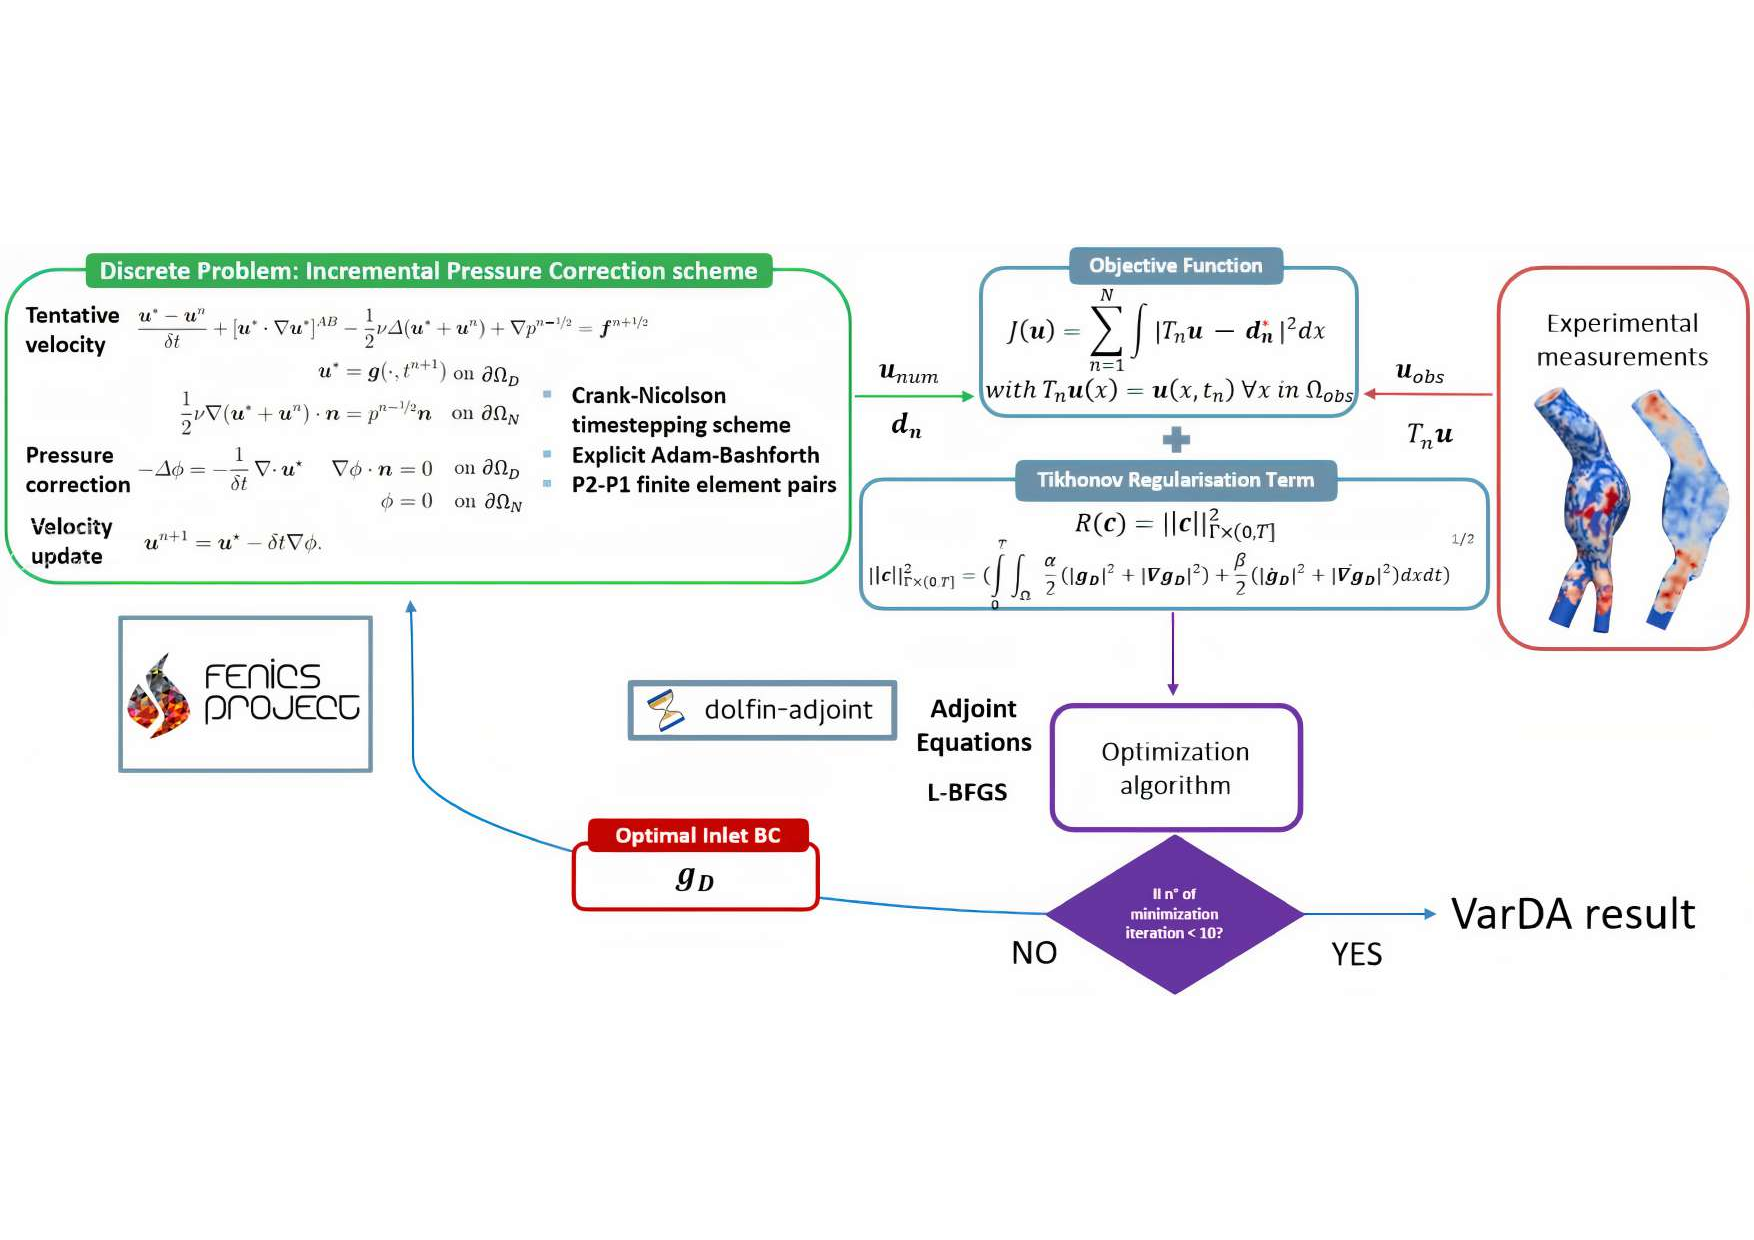
\includegraphics[width=0.95\textwidth]{chapters/paratico/Fig1.1.pdf}
    \caption{\small \textbf{Top-left}: The finite element (FE) solver computes the Navier-Stokes (NS) equations with an initial guess for the inlet boundary conditions (BCs); \textbf{Top-right}: experimental velocity measurements are taken at discrete points in the domain; \textbf{Center}: discrepancy between the computational fluid dynamics (CFD) velocity field and experimental data is minimized by iteratively refining inlet velocity profile with a gradient-based method.}
    \label{fig:scheme}
\end{figure}

Convergence was ensured through Wolfe conditions [\cite{Nocedal2006}], with maximum number of 10 iterations and ftol = $1 \times 10^{-9}$ and gtol = $1 \times 10^{-12}$ as tolerances.
The performances of the method were assessed by $J(\textbf{u})$ value before and after optimization, Root Mean Squared Error (RMSE) between \( \mathbf{u}\) and \( \mathbf{u}_{\text{obs}} \), and qualitative analysis of the effect on the velocity field through the software \emph{Paraview}.

\subsection*{Benchmark Tests}

\label{sec:bench}
\textbf{\textit{Preliminary tests}} - 
First, preliminary tests were performed to compare the computational efficiency of IPCS vs. an alternative coupled scheme [\cite{Figueroa2006}] in a 2D straight conduit (which represents a case of 2D VarDA and can thus be addressed using the term I defined as \emph{2DVar}). Simulations were run under laminar conditions at both low and high Reynolds numbers (Re), in order to evaluate the method in laminar and transitionally unstable regimes.  
The conduit was a longitudinal section of a cylinder with a diameter of 41 mm and a length of 200 mm, made of 4,967 mesh elements. Synthetic observations (\( \mathbf{u}_{\text{obs}} \)) were generated by an auxiliary CFD simulation, prescribing a parabolic velocity profile at the inlet with peak velocity \( U_{\text{max}} = 600 \, \text{mm/s} \) (Re = 6649) and with \( U_{\text{max}} = 50 \, \text{mm/s} \) (Re = 554) for turbulent and laminar conditions, respectively.
In the Tape, the tentative inlet velocity profile was parabolic with \( U_{\text{max}} = 800 \, \text{mm/s} \) (Re = 8865) and \( U_{\text{max}} = 100 \, \text{mm/s} \) (Re = 1108).
The iterative minimization of the discrepancy between \( \mathbf{u} \) and \( \mathbf{u}_{\text{obs}} \) was performed to determine the optimal velocity profile for CFD simulations, verifying if it matched the parabolic profile used to generate the synthetic observations.\\


\textbf{\textit{Progressively demanding tests}} - Next, the method was benchmarked through three progressively more demanding tests:

\begin{enumerate}
    \item 2D straight conduit in transient conditions (which represents a case of 2D VarDA also involving time and can thus be addressed using the term I defined as \emph{2DVar+t} benchmark) - This benchmark shared the same domain of the 2DVar benchmark. However, both the auxiliary simulation for the generation of the experimental observations and Tape consisted in a sequence of two transient simulations: in the first simulation, velocity was initially equal to 0 mm/s everywhere in the domain, and at the inlet a parabolic velocity profile was imposed, whose peak velocity increased linearly from 0 to \( \frac{ U_{\text{max}}}{2} \) over 0.3 s; in the second simulation, the velocity field computed by the first one was used as IC and the inlet velocity parabolic profile was scaled by the time-dependent function \( f(t) \):

\begin{equation}
\small
f(t) = 
\begin{cases}
\frac{U_{\text{max}}}{2}\cos\left(\frac{\pi}{T_s}\left(t - \frac{T_s}{2}\right)\right), & \text{if } t \leq T_s \\
\frac{U_{\text{max}}}{2}, & \text{if } T_s < t \leq T_d
\label{eq:13}
\end{cases}
\end{equation}

where \( T_s = 300 \) ms and \( T_d = 540 \) ms are cardiac cycle's systolic and diastolic phases [\cite{Katz1977}]. Besides determining the optimal velocity profile for CFD simulations, spatial and temporal regularization terms [\cref{eq:12}] were incorporated into the optimization process and subjected to a sensitivity analysis.\\

    \item 3D straight conduit in steady-state conditions (which represents a case of 3D VarDA and can thus be addressed using the term I defined as \emph{3DVar} benchmark) - This benchmark evaluated the computational cost increase when transitioning from a 2D to a 3D problem. The fluid domain was a 3D cylinder with a radius of 30 mm and a length of 200 mm, made of 74,968 mesh elements. IC and BCs, as well as the objective function, were identical to those in the 2DVar benchmark.
    \item Patient-specific AAA geometry in steady-state conditions (which represents a case of 3DVar applied to a patient-specific AAA geometry and can thus be addressed using the term I defined as AAA benchmark) - This benchmark aimed to test VarDA in a complex 3D domain using real experimental observations. 4D flow imaging was acquired from an adult male with AAA using a 3T coronary magnetic resonance (CMR) system (Ingenia, Philips Healthcare, Netherlands) at Linköping University Hospital. The 4D flow data were processed with in-house Python [\cite{Saitta2024}] and CMR angiography was performed for 3D AAA geometry segmentation.
Two tests were carried out with laminar flow in the AAA. In the first test, observations consisted in 4DFlow data acquired during early systole, corresponding to the third time frame (about 63 ms from the start of the cardiac cycle, with a 21 ms time step), while the Tape was generated by a CFD simulation fed by 4DFlow-based inlet velocity profiles. The second test assessed the method's robustness against noise, using an inlet velocity profile, scaled by 0.15, at peak systole to produce the Tape's output. Noisy observations were generated by processing the Tape's output according to medium noise setting of \cite{Saitta2024}.
In addition to already-mentioned metrics, wall shear stresses (WSSs) from final simulation we analyzed using custom Paraview filters.
\end{enumerate}

The associated codes can be found at the following link:
\textcolor{blue}{\url{https://github.com/saraparatico/proceedingsCodes/tree/main}.}

\section*{Results}
\label{sec:Results}
\label{ch:chapter_three}

\subsection*{Computational costs}
Numerical experiments were conducted on various setups: a workstation with 24 CPUs and 64 GB RAM for 2DVar and 3DVar and a high-performance computing system with 40 CPUs and 190 GB RAM for 2DVar+t and AAA benchmark. 2DVar took 30 minutes and 3DVar took 6 hours on 12 CPUs; on the other side, 6 hours were required for 2DVar+t and 17 hours for AAA benchmark.

\subsection*{Preliminary tests}
In high Reynolds number tests, IPCS optimization reduced RMSE from 142.60 mm/s to 6.70 mm/s, while the coupled scheme faced convergence issues. In low Reynolds conditions, IPCS proved to be five times faster than the coupled scheme and achieved a final RMSE of 1.76 mm/s compared to 4.22 mm/s for the coupled scheme.

\subsection*{Progressively Demanding Tests}
\textbf{\textit{2DVar + t benchmark}} - When a zero-velocity field was imposed as IC, the post-optimization velocity field showed inconsistencies with respect to the observations.
In particular, a high-velocity region just downstream of the inlet section was obtained, while low velocity values were computed in the rest of the domain.
Moreover, these tests did not yield improvements by changing \(\alpha\), and increasing \(\beta\) further worsened the performance (Fig. \ref{fig:3.3}).

\begin{figure}
    \centering
    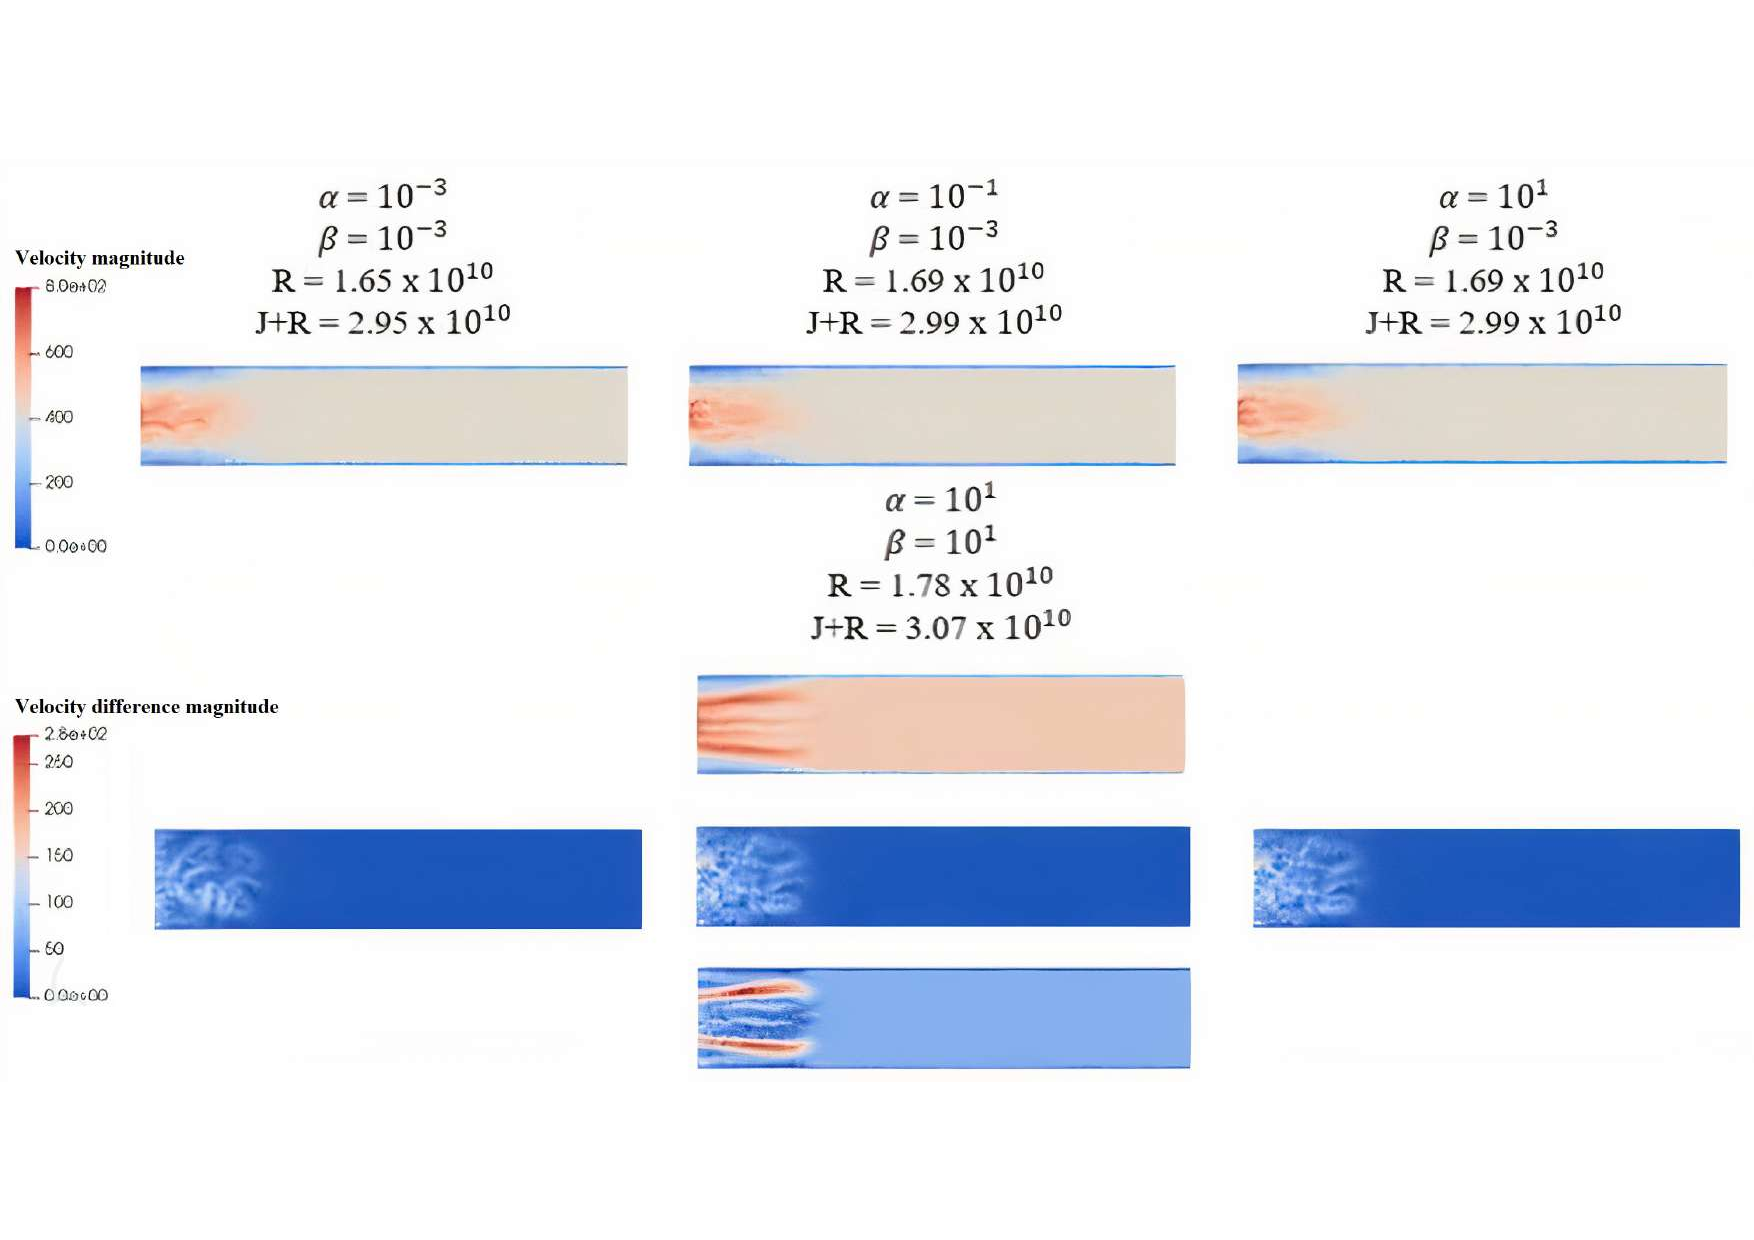
\includegraphics[width=\textwidth]{chapters/paratico/Fig1.2.pdf}
    \caption{Sensitivity analysis of regularization parameters at systolic peak. First row: 2DVar + t velocity magnitude for different $\alpha$ values ($10^{-3}$, $10^{-1}$, $10^{1}$), with $\beta = 10^{-3}$. Second row: test with $\beta = 10^{1}$ to assess time regularization. Third and fourth rows: velocity difference between reference and 3DVar results for each $\alpha$ and $\beta$.}
    \label{fig:3.3}
\end{figure}

When the initial velocity and pressure fields were set equal to those yielded by the previous post-optimization simulation, the results showed a more homogeneous flow better matching parabolic characteristics and with lower \(J + R\) values.\\

\textbf{\textit{3DVar benchmark}} - VarDA was performed with spatial regularization terms set to $\alpha = 10^{-2}$, $10^1$, and $10^3$. The lowest value of $J + R$ was achieved with $\alpha = 10^{-2}$, but it did not correspond to the lowest RMSE. The velocity field exhibited a peak near the inlet, suggesting continuity loss. For $\alpha = 10^1$, the lowest RMSE was achieved, and the post-optimization velocity field more accurately reflected the observed data. Increasing $\alpha$ to $10^3$ resulted in significant deviations from the observations, with unexpected velocity behaviors and higher values of $J + R$ and RMSE. This suggests that lower $\alpha$ values improve RMSE, while higher $\alpha$ values lead to smoother solutions, but can introduce inaccuracies when too large.\\


\textbf{\textit{AAA benchmark}} - In first tests, \(RMSE\) improved from 59.3 mm/s to 55.1 mm/s, indicating a better alignment with observations (Fig. \ref{fig:3.7a}). 
\begin{figure}
    \centering
    \begin{minipage}{\textwidth}
        \centering
        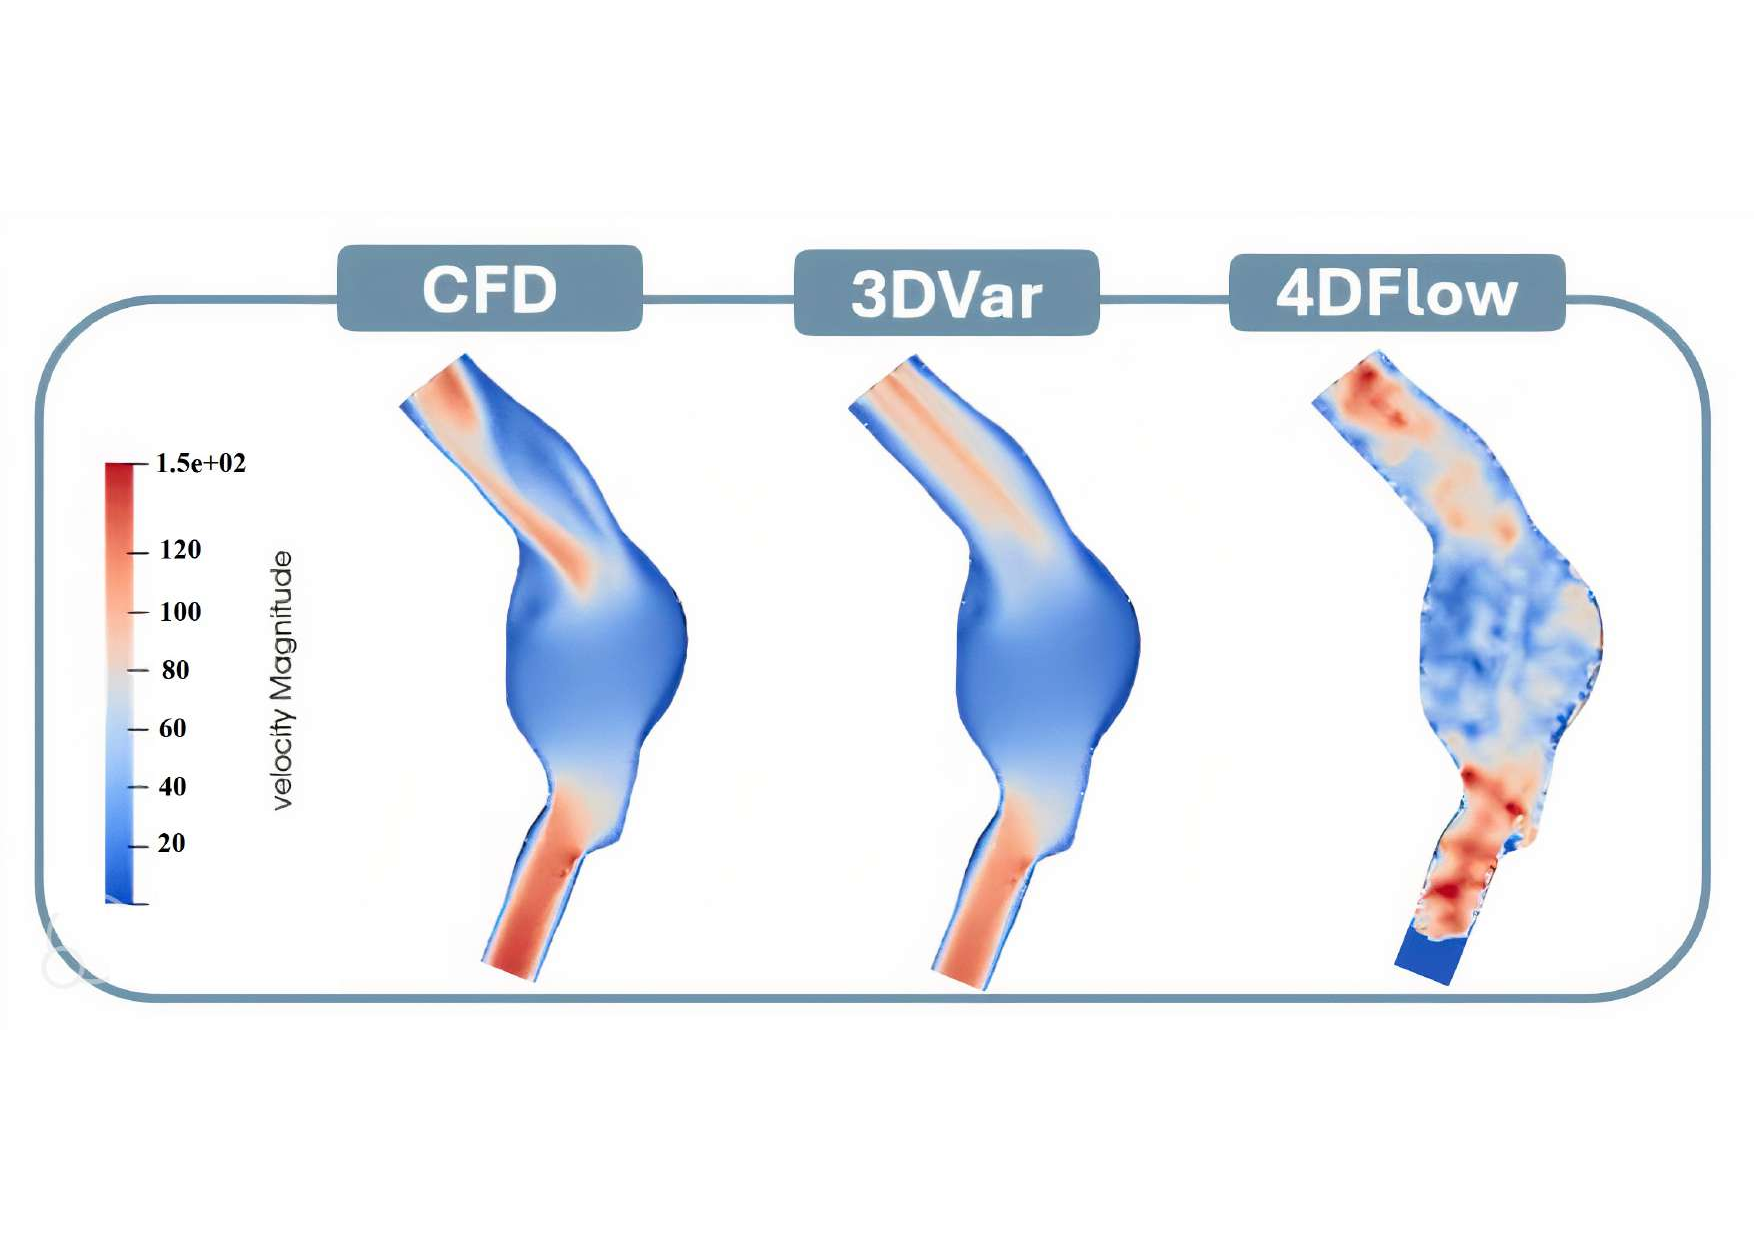
\includegraphics[width=0.9\textwidth]{chapters/paratico/Fig1.3a.pdf}
        \subcaption{\small AAA benchmark velocity magnitude maps.}
        \label{fig:3.7a}
    \end{minipage}
    \\[1em]  
    \begin{minipage}{\textwidth}
        \centering
        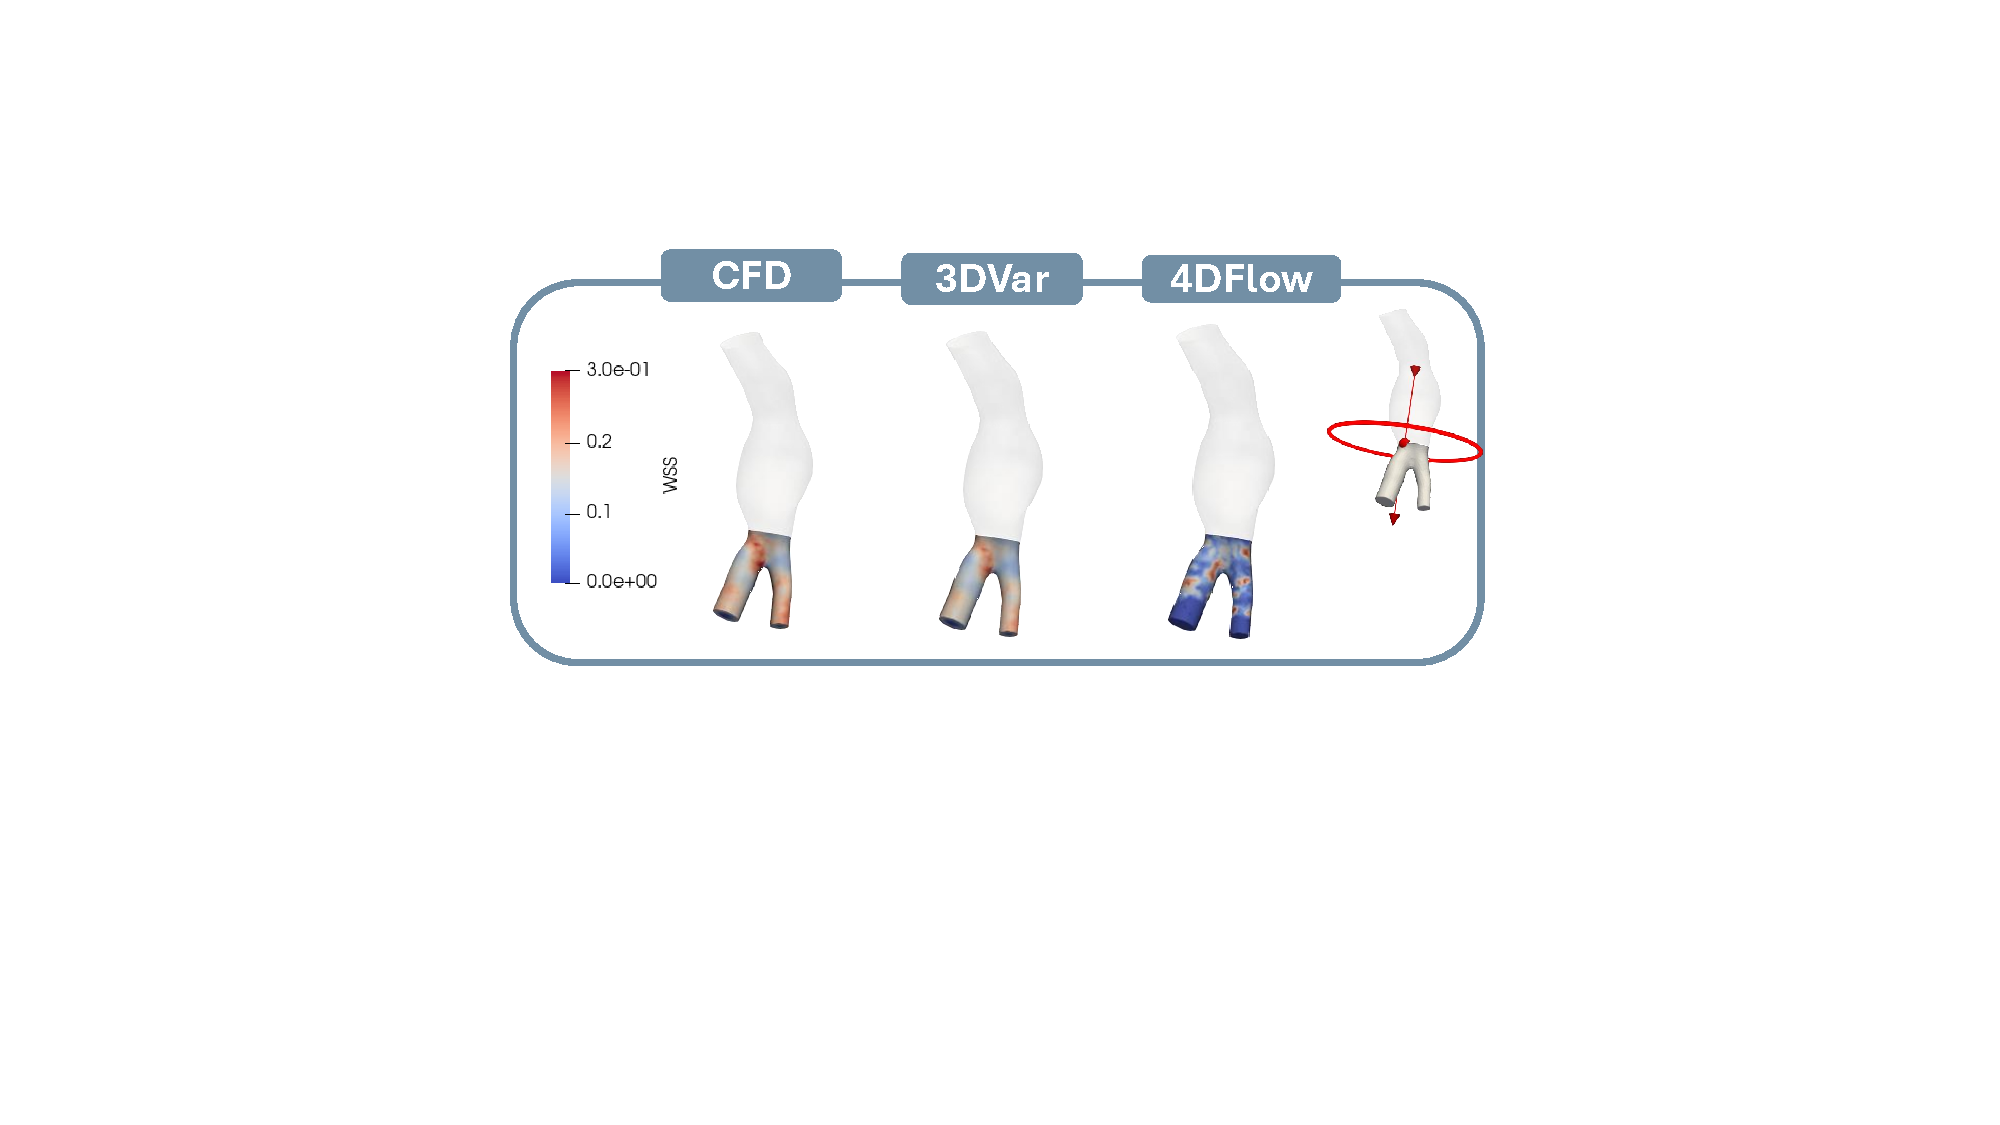
\includegraphics[width=0.9\textwidth]{chapters/paratico/Fig1.3b.pdf}
        \subcaption{\small AAA benchmark WSS maps.}
        \label{fig:3.7b}
    \end{minipage}
    \caption{\small (a) velocity and (b) wall shear stress (WSS) fields obtained on the abdominal aortic aneurysm (AAA) computed by computational fluid dynamics (CFD) (\textbf{left}), derived directly from 4DFlow MRI (\textbf{right}), and by  data assimilation (\textbf{centre}).}
    \label{fig:3.7}
\end{figure}

Generating a Tape took about 25 minutes, while optimization required 17 hours with 80 Gb of memory. WSS distributions from Tape's output and 3DVar predictions were consistent, identifying regions with high shear stress (Fig. \ref{fig:3.7b}). WSS distributions from Tape's output and 3DVar predictions were consistent in terms of location of high WSS regions. Moreover, while enforcing consistency with 4DFlow-based velocity measurements, the 3DVar method yielded a regular and realistic WSS distribution. This is a major difference as compared to the WSS distribution estimated directly from 4DFlow data, which was unrealistic owing to their poor space-resolution and to the impact of noise in the near-wall region. In tests with noisy observations, 3DVar effectively reconstructed the velocity field, slightly reducing \(RMSE\) from 36.8 mm/s to 36.4 mm/s, while maintaining WSS predictions consistent with CFD results, particularly at the iliac bifurcation, which is where the abdominal aorta splits into two smaller arteries, carrying blood to pelvis and legs.


\section*{Discussion}

\subsection*{From 2DVar+t to 3DVar}
The 2DVar+t reveals challenges due to inertial effects and short simulation durations, causing reconstruction defects from incomplete flow development. Extending simulation time for optimization is impractical due to high computational costs. A potential solution includes proper initialization of CFD simulations and implementing a checkpointing method to reduce computational costs by using only the last cardiac cycle for gradient calculations.
Moreover, a key difference between 2DVar+t and 3DVar is the flow field's response to regularization. In 2DVar+t, increasing $\alpha$ has minimal effect due to dominant time-dependent effects, reducing spatial regularization's impact. Additionally, increasing $\beta$ deteriorates the results, a challenge not present in 3DVar, emphasizing the difficulty of balancing temporal and spatial regularization in dynamic flows. Conversely, in 3DVar, moderate $\alpha$ values ($10^{1}$) significantly improve the velocity field, reducing inlet peaks and lowering \(RMSE\). However, excessive regularization ($\alpha = 10^{3}$) causes unrealistic velocity patterns. 

\subsection*{AAA benchmark}
AAA benchmark effectively reconstructs the velocity field in AAA geometry, maintaining high consistency with data obtained from 4D flow
imaging. It identifies high shear stress regions despite challenges due to lower resolution of 4D flow data near boundaries. The method remains robust against noise. 


\section*{Conclusions}
This study applies VarDA to estimate optimal inlet BCs for CFD using noisy 4D flow MRI data, minimizing mismatch with \textit{in vivo} velocity measurements.
The method yields a resolved, noise-free velocity field and is validated on 2D, 3D and patient-specific AAA geometries, demonstrating potential for personalized hemodynamic simulations.
The IPCS framework enhances efficiency and accuracy in transient flow analyses. Despite challenges in transient cases, this work lays the groundwork for future VarDA advancements with clinical implications.


\bibliographystyle{spbasic}
% Write the full path of your bibfile relative to book.tex
\bibliography{chapters/paratico/bibliography.bib}


